\documentclass[tikz,border=0pt,11pt]{standalone}
\usepackage[T1]{fontenc}
\usepackage[utf8]{inputenc}
\usepackage{lmodern,amsmath,amssymb}
\usepackage[swedish]{babel}
\usetikzlibrary{arrows.meta,calc,positioning,decorations.pathmorphing,decorations.pathreplacing,patterns,shadings}
\definecolor{navy}{HTML}{102F40}
\definecolor{teal}{HTML}{147D78}
\definecolor{lightteal}{HTML}{E6F1ED}
\definecolor{gold}{HTML}{B88B3B}
\definecolor{palegold}{HTML}{F7EEDB}
\definecolor{rust}{HTML}{B6533B}
\definecolor{palerust}{HTML}{FAEAE4}
\definecolor{paper}{HTML}{F7F5EE}
\definecolor{muted}{HTML}{5B6D72}
\definecolor{line}{HTML}{D6DED8}
\renewcommand{\familydefault}{\sfdefault}
\newcommand{\atom}[5]{\shade[ball color=#3!70] (#1,#2) circle (#5);\node[text=white,font=\bfseries\small] at (#1,#2){#4};}
\newcommand{\water}[3]{\begin{scope}[shift={(#1,#2)},scale=#3]\draw[navy!45,line width=2pt] (-.3,.22)--(0,0)--(.3,.22);\atom{0}{0}{rust}{O}{.22}\atom{-.3}{.22}{teal}{H}{.15}\atom{.3}{.22}{teal}{H}{.15}\end{scope}}
\newcommand{\panel}[4]{\filldraw[fill=white,draw=line,rounded corners=5pt] (#1,#2) rectangle ++(#3,#4);}
\newcommand{\note}[4]{\node[txt,text width=#3cm] at (#1,#2){#4};}
\tikzset{txt/.style={anchor=north west,align=left,text=navy,font=\small},
 head/.style={anchor=west,text=navy,font=\bfseries\large},
 label/.style={align=center,text=navy,font=\small},
 smalllabel/.style={align=center,text=muted,font=\footnotesize},
 arrow/.style={-{Latex[length=2.5mm,width=1.8mm]},line width=1.2pt,draw=teal},
 goldarrow/.style={-{Latex[length=2.5mm]},line width=1.2pt,draw=gold},
 rustarrow/.style={-{Latex[length=2.5mm]},line width=1.2pt,draw=rust},
 dashedarrow/.style={arrow,dashed},
 badge/.style={fill=lightteal,rounded corners=3pt,text=teal,font=\bfseries\small,inner sep=5pt}}
\begin{document}
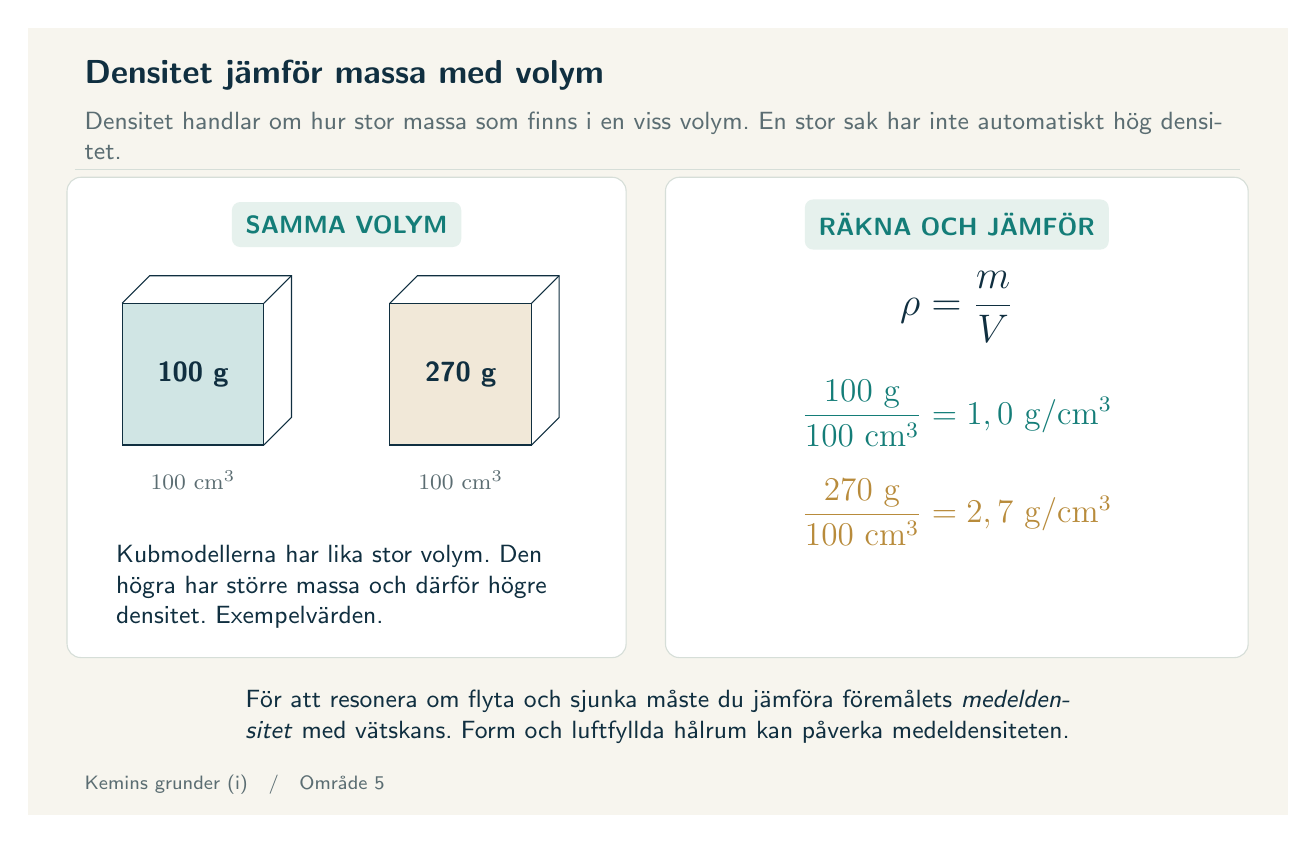
\begin{tikzpicture}[x=1cm,y=1cm]
\path[use as bounding box] (0,0) rectangle (16,10);
\fill[paper] (0,0) rectangle (16,10);
\node[head] at (.6,9.4){Densitet jämför massa med volym};
\note{.6}{9.05}{14.8}{\textcolor{muted}{Densitet handlar om hur stor massa som finns i en viss volym. En stor sak har inte automatiskt hög densitet.}}
\draw[line] (.6,8.2)--(15.4,8.2);

\panel{.5}{2}{7.1}{6.1}\panel{8.1}{2}{7.4}{6.1}
\node[badge] at (4.05,7.5){SAMMA VOLYM};\node[badge] at (11.8,7.5){RÄKNA OCH JÄMFÖR};
\foreach \x/\c/\m in {1.2/teal/100,4.6/gold/270}{\filldraw[draw=navy,fill=\c!20] (\x,4.7) rectangle++(1.8,1.8);\draw[navy] (\x,6.5)--++(.35,.35)--++(1.8,0)--++(0,-1.8)--++(-.35,-.35);\draw[navy] (\x+1.8,6.5)--++(.35,.35);\node[label,font=\bfseries] at (\x+.9,5.6){\m\ g};\node[smalllabel] at (\x+.9,4.25){$100\ \mathrm{cm^3}$};}
\node[label,font=\bfseries\Large] at (11.8,6.45){$\rho=\dfrac{m}{V}$};
\node[label,font=\large,text=teal] at (11.8,5.1){$\dfrac{100\ \mathrm{g}}{100\ \mathrm{cm^3}}=1,0\ \mathrm{g/cm^3}$};
\node[label,font=\large,text=gold] at (11.8,3.85){$\dfrac{270\ \mathrm{g}}{100\ \mathrm{cm^3}}=2,7\ \mathrm{g/cm^3}$};
\note{1}{3.55}{6.15}{Kubmodellerna har lika stor volym. Den högra har större massa och därför högre densitet. Exempelvärden.}
\node[label,text width=14cm] at (8,1.25){För att resonera om flyta och sjunka måste du jämföra föremålets \emph{medeldensitet} med vätskans. Form och luftfyllda hålrum kan påverka medeldensiteten.};\node[anchor=west,text=muted,font=\scriptsize] at (.6,.38){Kemins grunder (i)\quad /\quad Område 5};

\end{tikzpicture}\end{document}
